% Options for packages loaded elsewhere
\PassOptionsToPackage{unicode}{hyperref}
\PassOptionsToPackage{hyphens}{url}
\PassOptionsToPackage{dvipsnames,svgnames,x11names}{xcolor}
%
\documentclass[
  letterpaper,
  authoryear]{elsarticle}

\usepackage{amsmath,amssymb}
\usepackage{iftex}
\ifPDFTeX
  \usepackage[T1]{fontenc}
  \usepackage[utf8]{inputenc}
  \usepackage{textcomp} % provide euro and other symbols
\else % if luatex or xetex
  \usepackage{unicode-math}
  \defaultfontfeatures{Scale=MatchLowercase}
  \defaultfontfeatures[\rmfamily]{Ligatures=TeX,Scale=1}
\fi
\usepackage{lmodern}
\ifPDFTeX\else  
    % xetex/luatex font selection
\fi
% Use upquote if available, for straight quotes in verbatim environments
\IfFileExists{upquote.sty}{\usepackage{upquote}}{}
\IfFileExists{microtype.sty}{% use microtype if available
  \usepackage[]{microtype}
  \UseMicrotypeSet[protrusion]{basicmath} % disable protrusion for tt fonts
}{}
\makeatletter
\@ifundefined{KOMAClassName}{% if non-KOMA class
  \IfFileExists{parskip.sty}{%
    \usepackage{parskip}
  }{% else
    \setlength{\parindent}{0pt}
    \setlength{\parskip}{6pt plus 2pt minus 1pt}}
}{% if KOMA class
  \KOMAoptions{parskip=half}}
\makeatother
\usepackage{xcolor}
\setlength{\emergencystretch}{3em} % prevent overfull lines
\setcounter{secnumdepth}{5}
% Make \paragraph and \subparagraph free-standing
\ifx\paragraph\undefined\else
  \let\oldparagraph\paragraph
  \renewcommand{\paragraph}[1]{\oldparagraph{#1}\mbox{}}
\fi
\ifx\subparagraph\undefined\else
  \let\oldsubparagraph\subparagraph
  \renewcommand{\subparagraph}[1]{\oldsubparagraph{#1}\mbox{}}
\fi


\providecommand{\tightlist}{%
  \setlength{\itemsep}{0pt}\setlength{\parskip}{0pt}}\usepackage{longtable,booktabs,array}
\usepackage{calc} % for calculating minipage widths
% Correct order of tables after \paragraph or \subparagraph
\usepackage{etoolbox}
\makeatletter
\patchcmd\longtable{\par}{\if@noskipsec\mbox{}\fi\par}{}{}
\makeatother
% Allow footnotes in longtable head/foot
\IfFileExists{footnotehyper.sty}{\usepackage{footnotehyper}}{\usepackage{footnote}}
\makesavenoteenv{longtable}
\usepackage{graphicx}
\makeatletter
\def\maxwidth{\ifdim\Gin@nat@width>\linewidth\linewidth\else\Gin@nat@width\fi}
\def\maxheight{\ifdim\Gin@nat@height>\textheight\textheight\else\Gin@nat@height\fi}
\makeatother
% Scale images if necessary, so that they will not overflow the page
% margins by default, and it is still possible to overwrite the defaults
% using explicit options in \includegraphics[width, height, ...]{}
\setkeys{Gin}{width=\maxwidth,height=\maxheight,keepaspectratio}
% Set default figure placement to htbp
\makeatletter
\def\fps@figure{htbp}
\makeatother

% These are extra latex packages that the document depends on
% 
\usepackage{siunitx}
\usepackage{booktabs}
\usepackage{longtable}
\usepackage{array}
\usepackage{multirow}
\usepackage{wrapfig}
\usepackage{float}
\usepackage{colortbl}
\usepackage{pdflscape}
\usepackage{tabu}
\usepackage{threeparttable}
\usepackage{threeparttablex}
\usepackage[normalem]{ulem}
\usepackage{makecell}
\usepackage{xcolor}
\makeatletter
\makeatother
\makeatletter
\@ifpackageloaded{bookmark}{}{\usepackage{bookmark}}
\makeatother
\makeatletter
\@ifpackageloaded{caption}{}{\usepackage{caption}}
\AtBeginDocument{%
\ifdefined\contentsname
  \renewcommand*\contentsname{Table of contents}
\else
  \newcommand\contentsname{Table of contents}
\fi
\ifdefined\listfigurename
  \renewcommand*\listfigurename{List of Figures}
\else
  \newcommand\listfigurename{List of Figures}
\fi
\ifdefined\listtablename
  \renewcommand*\listtablename{List of Tables}
\else
  \newcommand\listtablename{List of Tables}
\fi
\ifdefined\figurename
  \renewcommand*\figurename{Figure}
\else
  \newcommand\figurename{Figure}
\fi
\ifdefined\tablename
  \renewcommand*\tablename{Table}
\else
  \newcommand\tablename{Table}
\fi
}
\@ifpackageloaded{float}{}{\usepackage{float}}
\floatstyle{ruled}
\@ifundefined{c@chapter}{\newfloat{codelisting}{h}{lop}}{\newfloat{codelisting}{h}{lop}[chapter]}
\floatname{codelisting}{Listing}
\newcommand*\listoflistings{\listof{codelisting}{List of Listings}}
\makeatother
\makeatletter
\@ifpackageloaded{caption}{}{\usepackage{caption}}
\@ifpackageloaded{subcaption}{}{\usepackage{subcaption}}
\makeatother
\makeatletter
\@ifpackageloaded{tcolorbox}{}{\usepackage[skins,breakable]{tcolorbox}}
\makeatother
\makeatletter
\@ifundefined{shadecolor}{\definecolor{shadecolor}{rgb}{.97, .97, .97}}
\makeatother
\makeatletter
\makeatother
\makeatletter
\makeatother
\journal{Transportation Research Part A}
\ifLuaTeX
  \usepackage{selnolig}  % disable illegal ligatures
\fi
\usepackage[]{natbib}
\bibliographystyle{elsarticle-harv}
\IfFileExists{bookmark.sty}{\usepackage{bookmark}}{\usepackage{hyperref}}
\IfFileExists{xurl.sty}{\usepackage{xurl}}{} % add URL line breaks if available
\urlstyle{same} % disable monospaced font for URLs
\hypersetup{
  pdftitle={Simulating Incident Management Team Response and Performance},
  pdfauthor={Gregory S. Macfarlane; Daniel Jarvis; Brynn Woolley},
  colorlinks=true,
  linkcolor={blue},
  filecolor={Maroon},
  citecolor={Blue},
  urlcolor={Blue},
  pdfcreator={LaTeX via pandoc}}

\setlength{\parindent}{6pt}
\begin{document}

\begin{frontmatter}
\title{Simulating Incident Management Team Response and Performance}
\author[1]{Gregory S. Macfarlane%
%
}
 \ead{gregmacfarlane@gmail.com} 
\author[2]{Daniel Jarvis%
%
}

\author[2]{Brynn Woolley%
%
}


\affiliation[1]{organization={Civil and Construction Engineering
Department, Brigham Young University},addressline={430
EB},city={Provo},postcode={84602},postcodesep={}}
\affiliation[2]{organization={Brigham Young University},addressline={430
EB},city={Provo},postcode={84602},postcodesep={}}

\cortext[cor1]{Corresponding author}



        
\begin{abstract}
The abstract is a crucial component of any scientific paper, as it
provides a summary of the research and its main findings. This paper
provides guidelines for writing an effective scientific abstract. The
first step is to identify the key elements of the research, such as the
research question, methods, results, and conclusions. Next, the abstract
should be written in a clear and concise manner, using simple language
and avoiding technical jargon. The abstract should also be structured,
with a clear introduction, methods section, results section, and
conclusion. Additionally, the abstract should accurately and succinctly
convey the main findings of the research, highlighting the significance
and implications of the work. By following these guidelines, researchers
can ensure that their abstract effectively communicates the key aspects
of their research and attracts the attention of potential readers. -
Written by ChatGPT
\end{abstract}





\end{frontmatter}
    \ifdefined\Shaded\renewenvironment{Shaded}{\begin{tcolorbox}[frame hidden, sharp corners, enhanced, borderline west={3pt}{0pt}{shadecolor}, interior hidden, boxrule=0pt, breakable]}{\end{tcolorbox}}\fi

\bookmarksetup{startatroot}

\hypertarget{introduction}{%
\section{Introduction}\label{introduction}}

Incident Management Teams (IMT) have become an integral strategy in
various regions to enhance highway system operations, particularly
during peak periods when user costs and roadway congestion can escalate
due to traffic incidents. These teams are adept at quickly addressing a
range of incidents, from minor vehicle breakdowns to severe multi-car
collisions, assisting other first response agencies in managing traffic
and restoring normal conditions.

Despite the substantial benefits and increasing reliance on IMT, there
is a notable gap in academic research, particularly in effectiveness
studies and prospective analyses that explore the potential impacts of
increased system deployment and the challenges posed by a rise in
traffic incidents. This could be attributed to factors such as driver
distraction, population growth, or other external influences. This
research aims to fill this gap, employing a mesoscopic-simulation
approach within the MATSim transportation modeling framework to
represent both incidents and IMT responses in a comprehensive manner.

Implemented in a scenario representing the Wasatch Front (Salt Lake
City) region of Utah, our study delves into the operational dynamics of
IMT, simulating various traffic incident scenarios to understand how
changes in resource allocation and incident concentration can influence
IMT effectiveness. Through a series of 20 simulations across three
distinct scenarios, we provide a detailed comparative analysis,
highlighting the potential for significant reductions in vehicle hours
of delay and improvements in traffic flow consistency.

This paper contributes to the existing body of knowledge on IMT,
offering insights into their operational dynamics and areas for
optimization. It underscores the importance of strategic IMT deployment
and the necessity for continuous evaluation and adaptation of IMT
strategies to meet the evolving demands of highway system operations.
The paper proceeds in a typical order. A discussion of previous research
into IMT motivations, effectiveness, and optimization follows this
introduction. \textbf{?@sec-methods} describes the simulation
methodology and scenario construction, while \textbf{?@sec-results}
presents the results of the analysis alongside a discussion of their
implications. The paper concludes in \textbf{?@sec-conclusion} with an
outline of future research motivated by this study's limitations.

\bookmarksetup{startatroot}

\hypertarget{sec-literature}{%
\section{Literature Review}\label{sec-literature}}

Traffic incident management in general --- and IMT in particular --- are
not strictly new innovations. The Federal Highway Administration (FHWA)
publishes the \emph{Traffic Incident Management Handbook} (FHWA, 2000),
which defines traffic incident management as:

\begin{quote}
\emph{The systematic, planned, and coordinated use of human,
institutional, mechanical, and technical resources to reduce the
duration and impact of incidents and improve the safety of motorists,
crash victims, and incident responders. (p.~1-1)}
\end{quote}

The handbook details the process of how to implement a traffic incident
management program as well as improve it. The manual covers various
aspects of incident management, including the responsibilities of
emergency medical teams, law enforcement, and other responding entities.
For this research, we focus on the dedicated traffic incident management
teams operated by departments of transportation or similar agencies and
not other types of first responders.

The FHWA has established performance measures to develop a framework to
quantify improvements to IMT operations and traffic (FHWA, 2000). Two
specific measures related to this research are: first, roadway clearance
time (RCT) is the time between the first recordable awareness of the
incident to the time all lanes open for traffic flow; second, incident
clearance time (ICT) is the time between the first recordable awareness
of the incident and when the last responder has left the scene.

Numerous studies have assessed the impact of Traffic Incident Management
(TIM) programs on traffic conditions, utilizing performance indicators
such as those provided by the Federal Highway Administration (FHWA). A
particularly noteworthy study conducted by \citet{schultz2019} explores
the relationship between the response times of Incident Management Teams
(IMT) and various traffic parameters, including roadway clearance time
(RCT), estimated travel time (ETT), and excess user cost (EUC). This
research leveraged interconnected data from the Utah Department of
Transportation (UDOT) and the Utah Highway Patrol, aiming to quantify
the traffic improvements resulting from swift IMT interventions at
accident sites. Analyzing 121 incidents, the study found that a
one-minute delay in IMT response correlated with a 0.8-minute increase
in RCT. This delay also impacted an additional 93 vehicles, added
roughly 34.6 minutes to the network's total estimated travel time, and
resulted in an extra \$925 in excess user costs. In essence,
\citet{schultz2019} established a clear connection between timely IMT
responses and improved traffic conditions, underscoring the importance
of rapid intervention.

\citet{kim2012}, in a study of Maryland's Coordinated Highways Action
Response Team (CHART) operations, devised a model using CHART's data to
compute the costs associated with traffic delay. The team established a
marginal cost-to-benefit ratio to discern the ideal fleet size. They
first estimated the reduction in traffic delay under various highway
response unit strategies. Subsequently, they calculated the costs of
fuel consumption, emissions, and delay times and converted these into
monetary values. These figures were then multiplied by the delay's
duration to obtain the traffic delay's marginal costs. The research
determined that each additional unit added provided a greater benefit
than its associated cost until seven highway response units were
deployed. This finding implies that while there is a significant
cost-to-benefit ratio with the optimal number of response teams, the
benefit diminishes when adding too many teams. Determining the ideal
number of teams is a function of budget, network size, and incident
frequency.

\citet{skabardonis1998} concluded in a study of the California Freeway
Service Patrol (FSP) IMT service that, on average, total incident
response time was 15 minutes longer when California Highway Patrol (CHP)
units responded without the support of IMT units. Using a system to
assign a cost per traveler per unit of time to vehicles in the observed
area, the authors determined that IMT units had a cost-to-benefit ratio
of 5:1. They also concluded that CHP officers spent less time on
incidents (including vehicle breakdowns) when assisted by incident
management team services.~

\hypertarget{imt-optimization}{%
\subsection{IMT Optimization}\label{imt-optimization}}

Given the evidence that IMT programs improve traffic conditions and
reduce costs for government entities and individuals, it becomes
paramount to further research avenues to maximize these benefits. One
effective strategy is the strategic placement of IMT units, optimizing
their spatial effectiveness to enhance their impact.

Enhancing IMT programs often focus on the precise deployment of
individual trucks and the strategic positioning of IMT
depots---locations where inactive trucks await dispatch. For scenarios
where IMT vehicles are actively on patrol, research often concerns
designing an efficient service area or ``beat.'' Various methodologies
have been applied to tackle this allocation challenge. While some
studies employ statistical models, incorporating a range of variables to
maximize specific performance measures given constraints, others opt for
digital modeling as a solution.

For instance, \citet{lou2011} explored strategies aimed at minimizing
IMT response time. They developed a mixed-integer nonlinear optimization
model and proposed different algorithms to address this problem. The
research modeled IMT units as roaming entities within specific freeway
sections, aiming to determine the optimal unit locations for minimizing
response times. Incident frequencies were generated randomly on the
network, given mean and standard deviations of incident occurrence on
each link in the network. The study focused on developing and optimizing
these algorithms for broad implementation rather than focusing on any
particular network or reducing response times in specific areas. They
implemented a template ``Sioux Falls'' network into the model as a
practical demonstration. Compared to the existing deployment plan in
Sioux Falls, the algorithm-generated plans could potentially reduce
total response time by 16.5-20.8\%.

\citet{ozbay2013} designed a mixed-integer programming model with
probabilistic constraints to optimize the allocation of Incident
Management Team (IMT) units across ``depots'' or staging areas in New
Jersey. This innovative approach, grounded in known probabilities of
various incident types, strategically positions IMT units to respond to
incidents, taking into account future probabilities on the network. The
primary goals were to minimize incident management costs and maximize
utility. The model was applied to a simplified South Jersey Highway
network, utilizing traffic incident data from the region to inform
demand distribution. Through this application, an optimal number of
depots and truck assignments were determined based on a \$500,000 budget
for the entire program. However, the lack of a comparative analysis with
pre-existing depot and unit distributions meant that the exact
improvements yielded by the model remained unquantified.

Digital models of IMTs have been developed in the past with various
software packages. \citet{pal2002} developed a digital model to
replicate IMT impacts on traffic conditions. Overall traffic time in the
system was used as the performance indicator of the units. The software
program was developed from scratch as existing programs at the time used
in mesoscopic traffic simulation could not simulate incident response
units. Various configurations of response vehicles were simulated using
probability distributions of crash data, vehicle speed, and carrying
capacity. Given the study results, suggestions were made regarding fleet
size, hours of operation, patrol area design, and improvements regarding
the dispatching policy.

These models, whether simulations and optimization problems, have served
their intended purposes effectively, but they fall short in mimicking
real-world scenarios as accurately as MATSim simulations do. Unlike
other models, MATSim allows for the integration of real-world data,
facilitating the creation of more realistic network simulations.
Additionally, it provides tools such as network change events and
within-day replanning, which contribute to a more accurate modeling of
driver behavior. These tools and their applications will be explored in
more detail in subsequent chapters.

An important consideration in determining the optimal location and fleet
size of IMT units is the metric by which the system is judged. The FHWA
has established performance measures by which IMTs were evaluated;
however, some researchers have felt that other metrics proved helpful in
specific scenarios. \citet{pal2002} use a metric of total traffic time
to analyze the model. Total traffic time is a practical approach as
traffic slowdowns incur financial costs and other burdens on the
individual and community \citep{bivina2016}. An economic cost-based
model is implemented in some research on incident management programs.
\citet{kim2012} use assumed values of fuel price and pollution
externalities gathered from previous research to assign a monetary value
to consequences of traffic delay in time and environmental costs. The
study focuses on optimizing IMT programs in general based on specific
budgets. Kim and Chang do not implement IMT units directly in their
traffic simulation. The total traffic time and financial costs are
similar in their fundamental nature in that financial costs are a
function of the traffic delay. From another perspective,
\citet{ozbay2013} developed a statistical model where the costs
associated with response times are minimized to meet budget constraints.
Deciding what factors are most important to measure in the traffic
simulation, like costs or response time, will help the decision-making
process behind IMT allocation.

\hypertarget{incident-modeling}{%
\subsection{Incident Modeling}\label{incident-modeling}}

As outlined in the preceding section, previous attempts to understand
optimal IMT deployment have been primarily based on ad-hoc models,
specially constructed utility functions, or similar stand-alone efforts.
Rarely has there been an explicit attempt to model traffic delay
associated with incident management, at least partially because research
modeling the effects of incidents on region-scale traffic networks is a
recent innovation.

Traffic models are based on static assignment, dynamic assignment, or
sometimes a combination of both. Static traffic assignment (STA) and
dynamic traffic assignment (DTA) make the same behavioral assumption:
drivers want to reach their destination in the shortest time possible. A
static model achieves optimization by calculating route travel times,
finding the shortest path, and adjusting routes toward equilibrium. The
issue with static models is that they assume that all vehicles
experience the same delay -- in particular, traffic flow is anisotropic
and obeys causality \citep{boyles2018}.

Dynamic modeling also aims to achieve equilibrium through route choice.
Dynamic modeling shows how congestion varies over time, and it bases
equilibration on experienced travel times, not instantaneous travel
times. According to \citet{boyles2018}, ``DTA is best applied when the
input data are known with high certainty, only a few scenarios are
needed, and detailed congestion and queueing information are critical''
\citep[ p.~28]{boyles2018}. A study on the effects of congestion
conducted by \citet{sisiopiku2007} highlighted the applications of
simulation-based DTA modeling on incident management. Her study argues
that dynamic assignment is preferred over static when considering
incident modeling. Sisiopiku describes her methodology as follows:

\begin{quote}
\emph{The overall approach in this study is to use the DTA capabilities
to support decision-making for incident management. Unlike static
assignment methods, which are based on average daily traffic and fail to
capture the dynamic process of an incident, DTA is particularly
appropriate for studying short-term planning applications such as
evaluating various incident management options (p.~111).}
\end{quote}

In this study, Sisiopiku used a simulation-based DTA model to assess the
impacts of designed incident scenarios. She evaluated the effectiveness
of candidate incident management plans and the impacts of traffic
operations and control strategies for the analysis period.

Sisiopiku initially conducted a base scenario under non-incidental
conditions, which served as a benchmark for comparison. The follow-up
scenario introduced an incident simulation, with the key caveat that
drivers were kept uninformed about the incident. The duration and
severity of the incidents were manipulated between different iterations
of this second scenario. The third scenario mirrored the second but
introduced information provision to the drivers. In this scenario,
drivers were empowered to optimize their route through the incident zone
and given access to information about pre-planned diversion paths. This
information was relayed to the drivers through Variable Message Signs
(VMS) strategically positioned upstream of decision points, as detailed
in Sisiopiku's 2007 study.

The scenarios Sisopiku ran in Birmingham and Chicago revealed that
travel time savings and traffic delay reduction could be achieved if
information was provided to the agents following an incident. The study
also shows how a simulation-based DTA model can simulate the impact of
incidents on congestion and the impacts of different traffic operation
and control strategies. The DTA tool Sisiopiku uses is Visual
Interactive System for Transport Algorithms or VISTA, a tool commonly
used in traffic modeling.

Echoing Sisiopiku's usage of VISTA, \citet{wirtz2005} also undertook an
in-depth analysis of this tool in his 2005 traffic incident simulation
study. Wirtz elaborated on the limitations of both VISTA and DTA
systems. As part of their route adjustment towards equilibrium, these
systems presume all drivers possess flawless travel time information for
routing to the user-optimal path. For instance, Sisiopiku, in her 2007
study, presumed a 100\% compliance rate for the diversion routes
provided to the drivers in her model. The validity of this assumption of
perfect travel time information is partially contingent on the
communication medium---radio traffic reports, the internet, or VMS.
Wirtz's 2005 study revealed that ``less-informed drivers spend more time
traveling than necessary, representing a departure from the user-optimal
traffic conditions simulated by VISTA.'' With the advancements in
personal GPS information and its increased accessibility, drivers are
more likely to identify an optimal path post-incident. It is critical to
acknowledge that the assumptions embedded in a model, along with its
scope and scale, significantly influence its functionality.

DTA models generally fall into two camps: microscopic and mesoscopic.
Microscopic models run on small scales and track the trajectories of
individuals. In contrast, mesoscopic models are more aggregated and
simplify variations in behavior; they involve elements of both static
modeling and dynamic microscopic models \citep{boyles2018}. The level of
detail in microscopic models makes them highly realistic but impractical
for modeling large regions. A mesoscopic model that shows the paths of
individual vehicles but ignores traffic flow issues like turn conflicts
and lane changes would work well for modeling traffic flow over a
greater area \citep{boyles2018}.

VISTA is an example of a mesoscopic model which showcases DTA's
capability for incident modeling. Microscopic models, like VISSIM, can
also be used for incident modeling. Microscopic models can track precise
locations of vehicles, driver behavior, and even vehicle
characteristics; this makes the models extraordinarily realistic but
impractical for modeling large regions \citep{boyles2018}. In Australia,
\citet{dia2006} used VISSIM to evaluate incident management impacts on
two arterial routes (Coronation Drive and Milton Road) connecting the
western suburbs of Brisbane and the Central Business District. Another
framework used for incident modeling is the traffic simulator JDSMART.
This model was used by \citet{vanlint2012} for incident simulation and
to study how roadway policies influence congestion.

MATSim, the Multi-Agent Transport Simulation Toolkit, has recently
gained recognition as a helpful software for incident modeling,
demonstrating a capacity for producing microscopic and mesoscopic
models. Operating as an open-source framework, MATSim is designed to
implement large-scale agent-based transport simulations. Using a
mesoscopic queue-based strategy, agents representing individuals seek
the shortest routes connecting their activities.

In his 2016 chapter of the MATSim manual, \citet{dobler2016} emphasized
the necessity and application of a within-day replanning tool within the
MATSim context. He elaborated that while MATSim's iterative modeling
approach fares well under ideal conditions and in achieving user
equilibrium, it falls short when dealing with unexpected occurrences.
This deficiency manifests as illogical behavior, such as preemptive
route changes before the incident's actual occurrence. For example,
Figure 1 illustrates a MATSim routing problem featuring within-day
replanning. It depicts an agent (a simulated individual) navigating from
the red dot to the green dot. A crash ensues along the agent's assigned
route at 14:02. Due to the iterative approach; however, the agent
switches to a different route at 14:00, two minutes before the crash.
This inconsistency exposes the limitations of an iterative approach in
modeling unanticipated behavior, underscoring the need for a within-day
replanning method, which utilizes a single iteration for replanning
rather than multiple.

\begin{figure}

{\centering 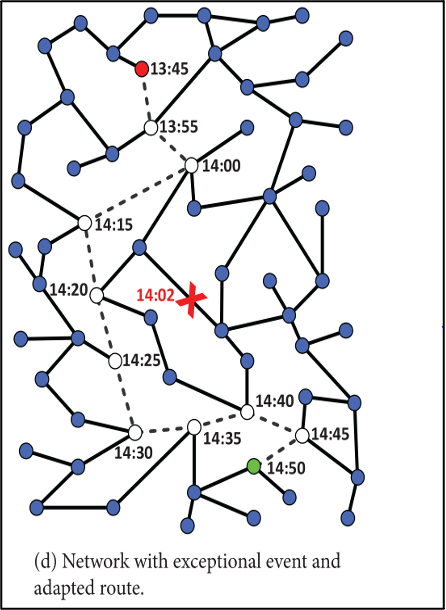
\includegraphics{figures/fig1.png}

}

\caption{Figure 1: Within-day replanning approach for a MATSim routing
problem.}

\end{figure}

While iterative systems leverage best-response modules, within-day
systems necessitate using a best-guess module. This approach means that
travel times can be optimized to a stable state with an iterative
approach, but this is not the case with a within-day approach. An
inherent attribute of within-day replanning is that it does not converge
to a user equilibrium, unlike an iterative process. Decisions, appearing
optimal in the moment, often reveal themselves as suboptimal upon
retrospective evaluation. Given the limited information available to the
agents in a within-day system, they may not necessarily choose the path
with the shortest travel time post-incident, as discussed by Dobler in
2016.

Replanning contains two categories: replanning an element of the
activity and executing the replanned elements. Elements include the
trip's start and end times, location, route, mode choice, or dropping of
a trip entirely. The system can execute plans for in-the-moment events
or those performed in the future. In a presently performed procedure, we
cannot conduct all replanning actions (e.g., we can no longer alter the
start time of an activity or the transport mode of a trip currently
being performed) \citep{dobler2016}. Figure 2: Iterative and within-day
replanning MATSim loop illustrates where within-day replanning fits
within a MATSim loop.

\begin{figure}

{\centering 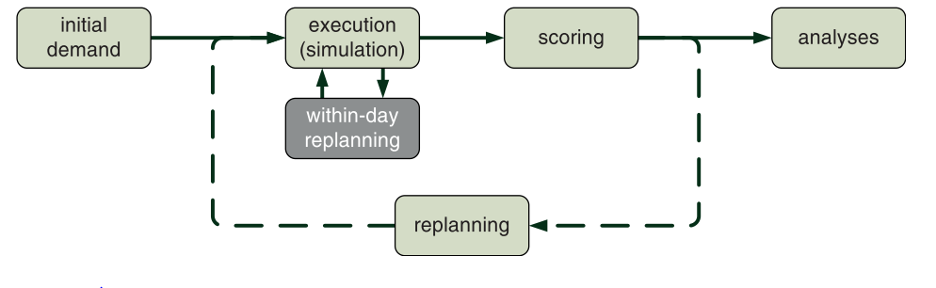
\includegraphics{figures/fig2.png}

}

\caption{Figure 2: Iterative and within-day replanning MATSim loop.}

\end{figure}

An alternative to iterative or within-day replanning only approaches is
to combine them. For example, we cannot thoroughly plan situations like
parking or car-sharing, requiring iterative and within-day replanning
methods. An agent can arrange a parking activity but cannot predict
which parking spots will be available when they arrive. Thus, we use
within-day replanning when the agent starts their parking choice.

In general, within-day or en-route replanning means that travelers
replan during the day or on their route, meaning that the simulation
needs to influence the agent while the network runs. \citet{dobler2016}
explains that we influence agents' decisions through loops or by having
users' routes dependent on the next link they choose. Because going
through all links and nodes at every step would be computationally
challenging, we may set certain links to be non-active and removed from
the computation \citep{dobler2016}. The two implementation methods
Dobler described are plan-based implementation and replacing the agent.

In a plan-based implementation, a loop is used where each agent can
deliberate in every time step. The agent can decide that they have
nothing to deliberate and return immediately. Because the number of
links is typically much smaller than the number of agents in a scenario,
massive optimization is necessary to make the loop computationally
efficient. For this reason, we could ask each agent to choose a link
only when they need to decide.

Such event-driven planning requires the agents to be re-programmed to
have enough capabilities to be oriented about themselves (i.e., be able
to compute plausible routes). Agents will only need to perform such
computation when replanning is triggered by an event like an emergency
warning or unexpected congestion; otherwise, they will follow their
usual daily plans.

Re-programing agents and implementing within-day replanning, as shown in
Figure 2: Iterative and within-day replanning MATSim loop., requires the
implantation of a \emph{MobsimEngine}, which can be plugged into the
mobility simulator seen in the execution phase of Figure 2: Iterative
and within-day replanning MATSim loop \citep{axhausen2016}.
\citet{dobler2016} describes it this way, ``in every simulated time
step, the QSim iterates over all registered \emph{MobsimEngines} and
allows them to simulate the current time step. Besides simulation of the
traffic flows, those engines can also let agents start or end
activities'' \citep[ p.~193]{dobler2016}. The engines contain within-day
replanning logic called \emph{WithinDayEngine}, which helps track agents
and adapt their plans \citep{dobler2016}. Not all agents need to compute
plausible routes at every turn, so an \emph{AgentSelector} selects the
agents to be replanned. \emph{AgentFilters} assist them in narrowing the
search population \citep{dobler2016}. Lastly,
\emph{TravelTimeCollectors} are part of the \emph{WithinDayEngine} and
provide actual link travel times to the replanners by collecting and
averaging travel times of agents that have recently passed a link during
a given time \citep{dobler2016}. The elements described above make up
the plan-based system.

A significant incident modeling, plan-based system study used MATSim to
simulate traffic incidents \citep{kaddoura2018}. Their research explains
that MATSim models transport users as individual agents. MATSim is
iterative and allows users to adjust travel plans during a single
iteration, from iteration to iteration, or both \citep{kaddoura2018}.
Kaddoura and Nagel accessed their incident data via the HERE application
programming interface for traffic incidents. This incident data included
Traffic Message Channel (TMC) information indicating an incident's cause
and severity. With such robust data, Kaddoura and Nagel could categorize
incidents as long or short-term and model each accordingly in MATSim.
Long-term effects include multiple-day lane closures, whereas short-term
incidents affect transport supply for less than a day. Their simulation
was based on an inner-city network in Berlin, Germany. Figure 3: Traffic
incidents mapped on the Berlin network illustrates the type of incidents
modeled and their severity. In this example, a crash on the southern
inner-city motorway ring road led to a full road closure, and several
construction sites caused partial capacity reductions.

\begin{figure}

{\centering 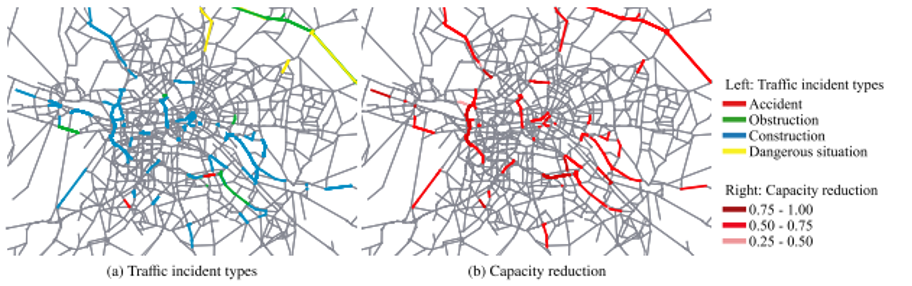
\includegraphics{figures/fig3.png}

}

\caption{Figure 3: Traffic incidents mapped on the Berlin network.}

\end{figure}

\citet{kaddoura2018} found that long-term traffic incidents increase
traffic congestion and the average car travel time by 313 sec (+18\%)
per trip. Short-term traffic incidents increase the average travel time
per car trip by another 136 sec (+8\%). Additionally, they found that
for 44\% of all car trips, the agent's transport route contained at
least one road segment for which the capacity or speed limit was reduced
because of an incident. Their study concluded that networks in which
transport users had high levels of knowledge about the incidents and
resulting traffic congestion still experienced an increase in travel
time caused by long and short-term incidents. Finally, Kaddoura and
Nagel asserted that ``accounting for traffic incidents makes the model
more realistic, allowing for an improved policy investigation'' \citep[
p.885]{kaddoura2018}. The modeling performed by Kaddoura and Nagel is
just one example of research on MATSim's capacity for incident-based
simulations.

A MATSim model developed by \citet{li2020} included various rescheduling
options, such as departure time, mode choice, and trip cancellation.
Their simulation found that if travelers received notice of an incident,
they would either depart early from their place of origin or switch to
public transport \citep{li2020}. The process proposed by Li and Ferguson
is beneficial because it allows agents to reassess their mode choice or
route assignment based on the notice of a reported incident. Li and
Ferguson show that users care about total travel time and travel time
variability (risk tolerance to a certain degree). The receiving of
notifications about incidents by agents impacted both factors. They
concluded that ``the provision of real-time traffic information is a
useful approach to mitigating the side-effects of incidents through
helping transport users efficiently adapt their day plans'' \citep[
p.96]{li2020}.

Additionally, they found that ``most of the travelers notified of being
affected by incidents are simulated to depart early or switch to public
transport, which effectively reduces the average travel time delay
caused by disruptions'' \citep[ p.96]{li2020}. Their findings validate
the conclusions of \citet{sisiopiku2007} that making incident
information available to agents leads to decreases in travel time and
congestion. Like the studies already mentioned, there have been various
modifications to and research on MATSim and its capacity.

In Thailand's capital, Bangkok, a study conducted by
\citet{peungnumsai2019} demonstrated the potency of the MATSim framework
in portraying the impact of rush hour congestion on select traffic
links. Peungnumsai ran various simulation iterations, loading the
selected links with a different number of agents: 10, 100, and 500. The
data collected and the subsequent analysis substantiated MATSim's
capability to demonstrate the congestion-induced variations in travel
time. Furthermore, it was observed that as the number of agents in the
simulation increased, there was a proportional surge in computing time,
physical memory usage, and the size of the output file. Despite the
scale of these simulations being relatively small, MATSim has the
capacity to simulate up to 10-100 million agents, encompassing various
modes of transportation like bicycles, motorbikes, cars, buses, and
taxis \citep{peungnumsai2019}.

In a contrasting study conducted in Copenhagen, Denmark,
\citet{paulsen2018} utilized MATSim to contrast the reliability of
automobile and railway travel times. His methodology involved using an
extension of MATSim centered around an event-based public transport
router, which facilitates optimal route selection for public transport
users by comparing the effectiveness of routes over several iterations.
Paulsen's simulation of travel times for both cars and trains yielded an
interesting finding: passenger delays were significantly influenced by
the adaptiveness of their chosen routes. However, he noted that
passenger travel times tended to be more unpredictable than trains,
which escalated with the degree of route adaptiveness. He concluded that
the adaptiveness of route selection contributed to significant travel
time fluctuations, a conclusion that aligns with the findings of
\citet{li2020}.

In essence, the studies encapsulated in Section 2.2 validate the
effectiveness of the open-source software MATSim, in simulating traffic
incidents, congestion, and travel times. This evidence accentuates how
the proper application of MATSim or similar Dynamic Traffic Assignment
(DTA) models can account for traffic incidents, thereby enhancing the
realism of the models. This type of model, in turn, can facilitate more
effective policy investigation, as noted by \citet{kaddoura2018}.

\hypertarget{summary}{%
\subsection{Summary}\label{summary}}

As explained in this section, there has been extensive research into
IMT's effectiveness and ability to restore traffic flow following long-
and short-term disturbances. Additionally, several studies have examined
how to effectively model traffic incidents and show their impact on
travel time, congestion, and mode choice. However, in these vast arrays
of findings, there is a gap in research on modeling IMT effectiveness
and incident impact on a loaded network with realistic agents. As a
result, it is difficult for researchers to understand how changes to
incident generation or IMT availability may impact traffic conditions.
In this research, we seek to combine these two strands, attempting to
model incident response in a mesoscopic simulation framework to bring
realism and detail to the IMT deployment question.

\bookmarksetup{startatroot}

\hypertarget{methodology}{%
\section{Methodology}\label{methodology}}

This section outlines the methods used for the Utah Incident Management
Team Optimization project model, building upon the main concepts
discussed in sections 2.1 and 2.2 of the literature review. The primary
goal of the model is to demonstrate the impact of traffic incidents on
overall traffic flow and assess the effectiveness of Incident Management
Teams (IMTs) within a simulated environment.

Our methodology is structured around three main components: setting up
IMT Vehicles and Incidents, understanding the functionality of the
MATSim model, and establishing scenarios for comparative analysis. In
the ``IMT Vehicle Configuration and Incident Selection'' section, we
define the origins of variables such as the size of the IMT fleet, their
initial placements, operational schedules, and specific details of
incidents, including location, severity, and frequency. These factors
are pivotal as they can significantly influence the network's
performance metrics. Following this, in the section on ``MATSim Model's
Functionality,'' we detail how these variables are integrated and
represented within the MATSim framework more closely align with
real-world conditions, building upon the foundational work of
\citet{kaddoura2018}.

Lastly, ``Scenario Simulations and Comparisons'' presents the range of
simulated scenarios used for comparison purposes. This section also
outlines the inputs for each scenario including the network, plans, and
configurations files used and their origins. The section explains the
comparative measures to be used in comparing scenarios against one
another which occurs in the results section of the report.

In the final subsection, ``Scenario Simulations and Comparisons,'' we
describe the assortment of scenarios that were simulated and the
rationale behind their selection. This part of the document describes
the specific inputs for each scenario, including the network, plans, and
configuration files, as well as their origins. Additionally, it details
the comparative measures employed to evaluate the scenarios against one
another, with a detailed analysis presented in the results section of
the report.

\hypertarget{imt-vehicle-configuration-and-incident-selection}{%
\subsection{IMT Vehicle Configuration and Incident
Selection}\label{imt-vehicle-configuration-and-incident-selection}}

The strategic placement and sizing of IMT fleets are pivotal in
optimizing vehicle response times, a relationship explored in depth by
\citet{lou2011} and \citet{pal2002}. Furthermore, \citet{schultz2019}
established a significant link between response time (RT) and roadway
clearance time (RCT). In the `IMT Vehicle Setup' subsection, we describe
the organization of the IMT vehicle, taking these relationships into
account and adhering to recommendations from Utah Highway Patrol
officials specific to this project.

Additionally, the nature and severity of incidents play a significant
role in affecting average travel times and delays, as evidenced by the
research of \citet{kaddoura2018}. The `Incident Data' and `Incident
Sampling' subsections elaborate on our methodology for selecting
incidents for the simulation scenarios, utilizing data from concurrent
research efforts.

\hypertarget{imt-vehicle-setup}{%
\subsubsection{IMT Vehicle Setup}\label{imt-vehicle-setup}}

The Utah Department of Transportation currently operates a fleet of 20
IMT vehicles, distributed across three zones corresponding to the
counties of Davis, Salt Lake, and Utah within the Wasatch Front.
Figure~\ref{fig-IMT_Map} visually represents the boundaries of each
county and the initial locations of both existing and newly proposed IMT
vehicles used in out simulated scenarios.

\begin{figure}

{\centering 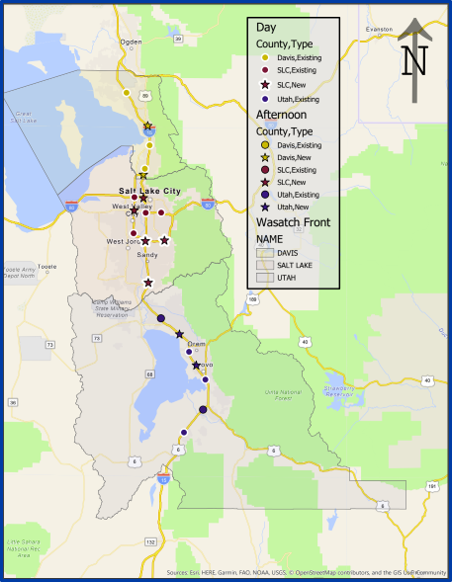
\includegraphics{figures/imt_map.png}

}

\caption{\label{fig-IMT_Map}IMT Starting Locations.}

\end{figure}

In this figure, circles represent existing vehicles, while stars denote
proposed additions. These starting locations aim to ensure a balanced
distribution across each county, based on shift types---either day or
afternoon. While this arrangement does not replicate the real-world
starting points of IMT truck drivers, who typically commence their
shifts from their homes, it is a pragmatic approach. Given that the
majority of their operations are concentrated along major interstates
such as I-15, I-80, and I-215, and considering the daily variability in
starting locations, positioning them along these primary routes is
logical for our MATSim Scenario simulations. Notably, the
``Increased-IMT'' scenario incorporates all vehicles from the
``Existing'' fleet, supplemented by an additional 10 vehicles
distributed across the three counties.

Our investigation primarily focuses on analyzing the potential impacts
of augmenting the IMT fleet, rather than the influence of their starting
locations. We hypothesize that an increase in vehicle numbers, assuming
an equitable distribution, could enhance IMT effectiveness.

Additionally, vehicle scheduling is a critical aspect of our setup. All
three counties operate IMT vehicles across day and afternoon shifts,
with specific timeframes detailed in the trucks file for MATSim scenario
runs. Although IMT vehicles typically do not cross county borders during
operations, our MATSim network does not impose such constraints,
allowing for vehicle movement across counties based on incident
proximity. With these vehicle configurations established, we now turn
our attention to the incident data the sampling used in establishing
simulated scenarios.

\hypertarget{incident-data}{%
\subsubsection{Incident Data}\label{incident-data}}

Joel Hyer, a student at Brigham Young University, conducted concurrent
research to acquire a dataset of incidents having received Utah Incident
Management Team (IMT) intervention, sourcing data from TransSuite and
the Utah Highway Patrol. He ensured that each incident record in the
dataset was complete, providing essential details such as start and end
times (with the latter derived from the Roadway Clearance Time (RCT)),
location, and the degree of capacity reduction.

From the data collected in 2018 and 2022, Joel compiled a comprehensive
list of 411 unique incidents, ranging in severity from property damage
to fatal accidents. This dataset served as the foundation for selecting
incidents to include in the MATSim model. However, it is important to
note that this list does not represent the total number of incidents
responded to by UHP and IMT services. The `master list' contains all
incidents responded to by the Utah Highway Patrol and provides a more
accurate depiction of daily incidents. Even still, it is important to
acknowledge that both data sets only include incidents that received a
response from UHP or IMT services, omitting those that did not.

\hypertarget{incident-sampling}{%
\subsubsection{Incident Sampling}\label{incident-sampling}}

To accurately model the daily frequency of incidents, we conducted a
thorough analysis of the `master list' of incident data, from which we
derived a distribution of incident count frequencies to inform our
sampling methodology.

We employed the Pandas library in Python to create a script that imports
the data into a data frame, eliminates any duplicate entries, and
refines the `Call Received Time' and `Call Type' columns. We then
aggregated the data by date and call type, counted the incidents, and
generated a new data frame that details the daily frequency of
incidents. These frequencies served as the foundation for creating a
weighted distribution, which in turn facilitated our sampling process.
To ensure consistency and replicability of our results, we integrated a
fixed random seed value into our script. This setup allowed us to
perform random sampling, extracting ten days from the incident number
distribution based on the established frequencies. These ten values were
then utilized to simulate ten scenarios based on observed or current
incident frequencies.

Utilizing the incident data, we established a total of 20 scenarios,
categorized into two distinct groups: Current Incident Frequencies and
Increased Incident Frequencies. For the scenarios under Current Incident
Frequencies, we employed the script described above to select ten days
from a weighted sampling distribution, which determined the number of
incidents to be simulated for each respective day. On the other hand,
the scenarios categorized as Increased Incident Frequencies were
designed to evaluate the resilience and performance of the IMT system
when confronted with a substantial increase in daily incidents. Drawing
from the upper range of the 2022 data, we identified days with incident
counts varying from 18 to 21. To ensure a thorough and comprehensive
evaluation, we decided to simulate additional days for each incident
count, resulting in a distribution of two days with 21 incidents, two
days with 20 incidents, three days with 19 incidents, and three days
with 18 incidents. Figure~\ref{fig-Inc_Map} visually represents the
original distribution of daily incidents, as well as the distributions
for both current and increased incident frequencies used in assigning
the number of incidents to each simulation scenario.

\begin{figure}

{\centering 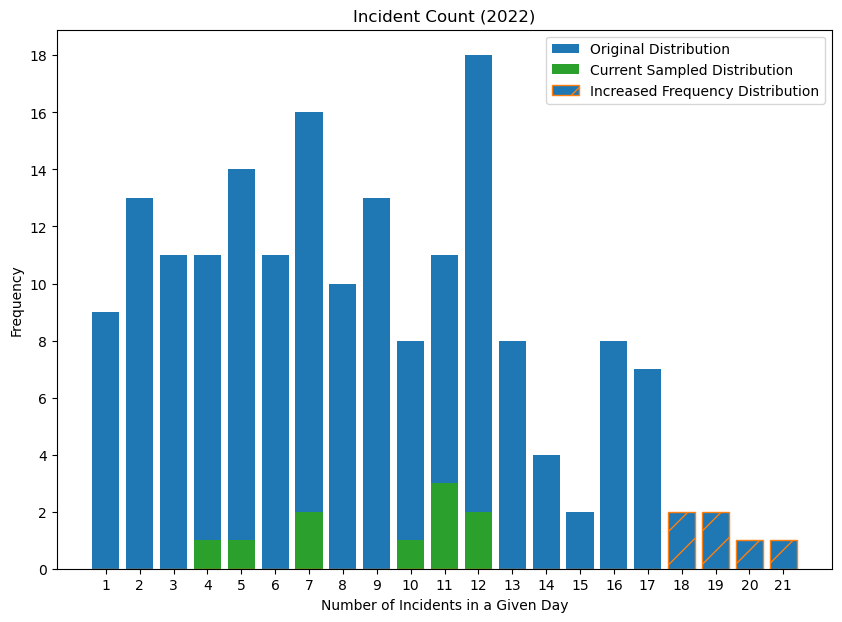
\includegraphics{figures/inc_sampling.png}

}

\caption{\label{fig-Inc_Map}Figure 5: Incident Sampling.}

\end{figure}

Upon determining the distribution of incidents for each scenario, we
assigned a three-digit seed value to each of the twenty scenario
groupings, serving both as an identifier and a tool for incident
selection. Within MATSim, each scenario received a specified number of
incidents and a seed value. Utilizing these parameters, a number of
incidents `X' was randomly selected from the list of 411 incidents,
ensuring that the same incident did not occur more than once within a
single simulation. For future research, additional parameters could be
established for incident selection to ensure the creation of logical and
realistic incident scenarios.

\hypertarget{matsim-functionality}{%
\subsection{MATSim Functionality}\label{matsim-functionality}}

In the MATSim model, factors such as incident selection are programmed
within the model. The distribution and scheduling of trucks are
described in XML truck files, which are then loaded into the model. As
highlighted in the literature review, MATSim is an open-source platform
that consists of various modules and packages. These components can be
created, imported, and edited by users across the platform, fostering a
collaborative environment.

For the purposes of our research, we developed the ImtModule, a
specialized package designed to process incidents and IMT responses
within the simulation. This module leverages existing research on
incident simulation, Demand Rapid Transit (DRT), event handling, and
vehicle dispatch algorithms, building upon these foundations to enhance
the functionality of our model.

In this section, we delve into some of the specific tools within MATSim
that we utilized and adapted to construct a comprehensive and functional
model for both processing and analysis. These tools include Network
Change Events, Vehicle Assignment, and Incident Response. Together, they
contribute to the realism and precision of our traffic simulations,
particularly in the context of responding to roadway incidents, ensuring
that our model provides accurate and reliable results.

\hypertarget{network-change-events}{%
\subsubsection{Network Change Events}\label{network-change-events}}

In a MATSim network, each link is characterized by specific attributes
such as type, length, number of lanes, free-flow speed, and capacity. To
effectively simulate unexpected events and their subsequent impacts on
traffic flow, it is essential to dynamically adjust these attributes.
This capability, termed a Time-Dependent Network, is elaborated upon in
the MATSim textbook and is vital for ensuring the realism and accuracy
of our simulation.

Network Change Events (NCEs) serve as the mechanism within MATSim for
modifying network attributes at precise moments during a simulation.
Detailed in Section 6.1 of the MATSim textbook, the implementation of
NCEs necessitates specific adjustments to the MATSim configuration file
to facilitate a time-variant network. These events can modify a link's
free-flow speed, number of lanes, or capacity. To initiate a network
change event, the system requires specific information including the
time of the event (startTime), the affected link(s) (link refID), the
type of change (free-flow speed, lanes, or capacity), and the value of
the change.

Implementing network change events for incidents in our simulation is
relatively straightforward. Each incident is specified with a start
time, link ID, and capacity reduction factor. However, triggering
network change events upon the arrival of an IMT vehicle is a more
complex task. As outlined in the `Vehicle Assignment' section, IMT
vehicles are dispatched similarly to taxis or ambulances, building upon
the existing framework of Demand Rapid Transit (DRT) described in the
MATSim textbook. In line with their assignment algorithm, IMT vehicles
receive a request and proceed to the location of the affected link.
Their arrival times are variable and depend on the current traffic
conditions.

To manage this uncertainty, we employ an `event-handler', a tool that
records the events of a simulation as it progresses. These events
provide insights into when specific vehicles enter and exit links en
route to their destinations. For IMT vehicles, event handlers were
utilized to monitor their arrival at incident links, triggering specific
network change events. In this study, every time an IMT vehicle reached
an impacted link, it restored 25\% of the link's lost capacity.

This approach ensures a dynamic and responsive simulation, reflecting
the real-world scenarios where IMT vehicles play a crucial role in
mitigating the impacts of roadway incidents. The implementation of the
MATSim within-day replanning module further enhances this
responsiveness, enabling the rerouting of other agents on the road in
the aftermath of an incident.

Contrary to the work of \citet{kaddoura2018}, our study does not take
into account long-term capacity reduction events such as road
construction, focusing exclusively on short-term incidents like
accidents or vehicle breakdowns. The reduced capacity of a specific link
generally impacts all agents, both regular and IMT vehicles. However, if
a subnetwork is employed, IMT trucks, akin to other emergency vehicles
such as ambulances and firetrucks, experience less disruption from
congestion caused by daily traffic or unexpected incidents.

\hypertarget{within-day-replanning}{%
\subsubsection{Within-Day Replanning}\label{within-day-replanning}}

\textless\textless{} The model was meant to incorporates the concept of
within-day replanning to a certain extent, as elaborated in Chapter 30
of the MATSim textbook. I loaded the within-day replanning module but
didn't specify which agents needed to use it or the times that they
needed to use it. \textgreater\textgreater{}

\textless\textless{} Dr.~Macfarlane. Within-day replanning is not being
implemented in the way that I thought that it was. After re-reading the
literature review I realized that I had confused the replanning that
occurs from iteration to iteration with the replanning mentioned by
\citet{kaddoura2018} that only occurs for specific agents within the
simulation. \textgreater\textgreater{}

\textless\textless{} I do think it is still worth mentioning their
research, and I can discuss how we could have used within-day replanning
more effectively in the limitations section of this report. I am sorry
for the confusion and for not realizing the problem earlier. Perhaps
this section in the Methodology could discuss the strategy the model
uses from iteration to iteration. \textgreater\textgreater{}

\textless\textless{} I'll likely move this section to the limitations
and talk about it, but wanted to leave you a note here just in case you
were looking for this section - Daniel Jarvis\textgreater\textgreater{}

\hypertarget{vehicle-assignment}{%
\subsubsection{Vehicle Assignment}\label{vehicle-assignment}}

In the MATSim simulation, the dispatch of one or more Incident
Management Team (IMT) vehicles is triggered when an incident occurs. The
selection of the most appropriate IMT vehicle for the task is determined
by a dispatch algorithm. This algorithm may base its decision on either
a least-cost path calculation, which takes into account factors such as
congestion and link speed, or it may opt for the shortest path between
the vehicle's current location and the incident site. The effectiveness
of these methods is contingent upon the IMT units' ability to navigate
through traffic. In scenarios where a subnetwork is employed, IMT
trucks, like other emergency vehicles, are less impacted by congestion
and variations in free-flow speed. This could render the shortest path
calculation a more viable option. On the other hand, if IMT vehicles are
subject to the same traffic conditions as regular vehicles, a least-cost
path calculation might be the more prudent choice within the simulation.

In this project, the Utah IMT system operates collaboratively with the
Utah Highway Patrol, sharing a common dispatch service. IMT vehicles,
equipped with sirens and flashing lights similar to those on highway
patrol vehicles, are assigned to specific zones and have the capability
to navigate through traffic like other emergency vehicles. Given this
capability, the dispatch system prioritizes the IMT vehicle that can
reach the incident site most efficiently, taking into account the
current traffic conditions. This operational protocol ensures that,
within the simulated scenarios, the IMT vehicle selected is not merely
the closest in terms of distance, but also the most strategically
positioned to respond swiftly and effectively.

Upon arrival at an incident site, IMT vehicles play a crucial role,
primarily through their interaction with Network Change Events (NCEs)
within the ongoing simulation. They utilize the same mechanisms as
incidents to effect changes in the network, contributing to the dynamic
and responsive nature of the simulation. This ensures that the
simulation remains a valuable tool for understanding and planning for
real-world scenarios, particularly those involving roadway incidents and
the subsequent deployment of IMT vehicles.

It is important to note that resource limitations may sometimes restrict
the number of IMT units available to respond to an incident. In
instances where an incident would ideally be managed by 2 or 3 IMT
units, only a single vehicle might be dispatched, potentially leading to
extended management or cleanup times. This limitation, along with its
implications, will be discussed in more detail in the conclusion and
limitations section of this report.

\hypertarget{incident-response}{%
\subsubsection{Incident Response}\label{incident-response}}

Network Change Events (NCEs) play a crucial role in the MATSim network,
simulating the effects of incidents on agents and demonstrating how
these events impact user behavior. Additionally, NCEs highlight the
influence of Incident Management Teams (IMTs) on agents' travel times
and paths, providing a comprehensive view of incident response.

Upon the occurrence of an incident, the vehicle assignment algorithm is
tasked with dispatching IMT units, leading to a critical decision: what
impact will the IMT vehicles have on the affected links? Two primary
strategies are considered:

\begin{enumerate}
\def\labelenumi{\arabic{enumi}.}
\tightlist
\item
  Incident Duration Reduction: The IMT vehicles can decrease the
  duration for which the link's capacity is reduced, effectively
  shortening the incident's length.
\item
  Capacity Restoration: Upon their arrival, IMT vehicles can restore a
  certain percentage of the link's lost capacity.
\end{enumerate}

The decision between these strategies is dependent on the data available
to the user. In the context of this project there is a lack of
comprehensive data comparing incidents with and without IMT or highway
patrol intervention. This data gap, highlighted in our literature
review, prevents an accurate prediction of an incident's potential
duration without external assistance and hinders informed
decision-making in incident management.

In the absence of clear comparative data, the practicality of the first
option---incident duration reduction---remains uncertain. However, this
study has adopted the second strategy, capacity restoration, with IMT
vehicles restoring 25\% of the capacity gap on an incident link upon
their arrival. This capacity gap is defined as the difference between a
link's full capacity and its reduced capacity during an incident.

Figure~\ref{fig-Cap_Restore} visually represents the potential impact of
an incident without IMT intervention, contrasting it with scenarios
involving the response of one or two IMT units. This illustration
underscores the significance of IMT vehicles in incident management and
their potential to mitigate the effects of incidents on network traffic
flow.

\begin{figure}

{\centering 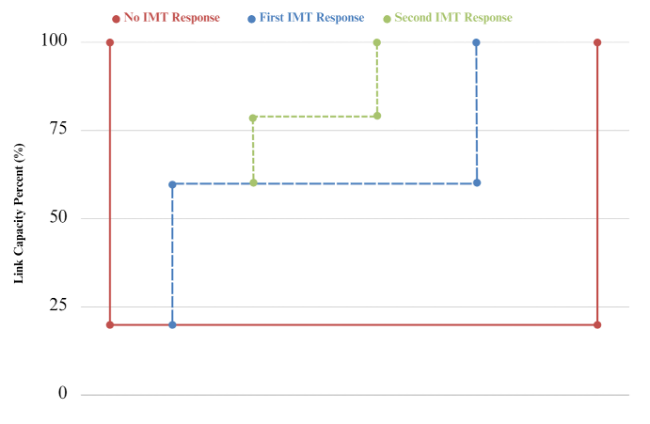
\includegraphics{figures/cap_restore.png}

}

\caption{\label{fig-Cap_Restore}Figure 4: IMT Capacity Restoration Upon
Arrival.}

\end{figure}

\hypertarget{scenario-simulations-and-comparisons}{%
\subsection{Scenario Simulations and
Comparisons}\label{scenario-simulations-and-comparisons}}

Given the context regarding incident selection, IMT organization, and
their collective impact on a network and its agents, a series of
simulation scenarios were designed for a comprehensive comparative
analysis. Each scenario was executed using a network and plans file
previously utilized in research conducted by Dr.~Macfarlane and research
students at Brigham Young University for the Wasatch Front Regional
Council (WFRC).

These network and plans files were integrated into our simulation
scenarios, alongside the ImtModule described earlier, and other
configuration parameters. The config parameters were primarily
established by the configuration settings employed by
\citet{kaddoura2018} in their MATSim incident simulations. With all
parameters set up and organized, a total of 60 simulation scenarios were
executed to facilitate a thorough comparative analysis. The subsequent
section provides a detailed outline of these scenarios and the
methodology employed to compare and contrast their respective outcomes.

\hypertarget{incident-imt-scenario}{%
\subsubsection{Incident \& IMT Scenario}\label{incident-imt-scenario}}

This section outlines the methodology employed for selecting incidents
in a set of 20 simulated ``days.'' These simulations are categorized
into two distinct groups: one reflecting the current distribution of
incidents managed by the Utah Highway Patrol, and another representing a
10-day period with an elevated frequency of incidents, based on the
upper range of daily incident data gathered in 2022.

Each of the 20 scenarios was assigned a unique random seed value,
ensuring variability in incident selection across simulations.
Subsequently, each group of scenarios was further divided into three
distinct simulation conditions. The first condition, referred to as
``Incidents-Only,'' includes only the incidents without any IMT
intervention. The second condition incorporates the incidents along with
the deployment of 20 IMT vehicles, while the third condition includes
the incidents and an increased fleet of 30 IMT vehicles. For ease of
organization and comparison, each scenario was assigned a unique code,
such as ``1-10-257.'' In this coding system, the first digit denotes the
scenario type (Incidents-Only, 20 IMTs, or 30 IMTs), the second digit
represents the number of incidents included in the simulation, and the
third digit corresponds to the seed value used for random incident
selection. In total, seven overarching scenario groups were established,
as outlined below:

1. An incidents only scenario with no IMTs and current incident
frequency.

2. An incidents only scenario with no IMTs and increased incident
frequency.

3. Current IMT resources (20 vehicles) with current incident frequency.

4. Current IMT resources (20 vehicles) with increased incident
frequency.

5. Increased IMT resources (30 vehicles) with the current frequency of
incidents.

6. Increased IMT resources (30 vehicles) with the increased frequency of
incidents.

7. A baseline with no IMTs and no Incidents.

It is important to note, as described in the IMT Vehicle Setup section,
that not all IMT vehicles are operational simultaneously. Due to
scheduling constraints, the actual number of vehicles on the road at any
given time is typically approximately half of the total fleet size.

\textless\textless{} Brynn has prepared a table detailing these
different scenario types, which we could include here if desired.
\textgreater\textgreater{}

\hypertarget{comparative-measures}{%
\subsubsection{Comparative Measures}\label{comparative-measures}}

The study employed the MATSim model for simulations across three
scenarios: `Incidents', `20-Truck', and `30-Truck'. Each scenario was
compared internally, as well as against a `Baseline' scenario without
incidents or IMT intervention. This multi-level comparison provides an
overall view of the IMTs' influence on traffic flow and their
operational efficiency.

The primary metric for traffic impact analysis in this study is the
total vehicle hours of delay (VHD), dissected through three
investigative tiers: Network Links, Motorway Links, and Impacted Links.
`Network Links' offer a macroscopic view of the network-wide delay,
`Motorway Links' focus on major highways and freeways, and `Impacted
Links' provide a microscopic view of the delays at incident sites and
their immediate upstream links. This tiered approach ensures a thorough
analysis, capturing the overarching impact on traffic flow while also
honing in on critical areas affected by incidents. The comparative
analysis across different scenarios and tiers highlights the general
impacts of IMTs and their efficacy, particularly at the `Impact Link'
level.

In addition to VHD, the study investigates the performance and
operational efficiency of IMT vehicles. Metrics such as average travel
times, distances, and incident response times of IMT trucks are compared
across scenarios. The `20-Truck' scenario reflects the current fleet of
IMT vehicles, while the `30-Truck' scenario introduces an additional 10
vehicles, providing a basis for comparison to discern the impact of
fleet size on operational efficiency. The analysis encompasses both the
time and distance traveled by IMT trucks to incidents, offering insights
into how effectively these resources are deployed and utilized.

By comparing the performance metrics of IMT trucks across different
scenarios, we gain a better understanding of how fleet size influences
operational efficiency. This, in turn, informs strategic decisions
regarding resource allocation and deployment, ensuring that IMT vehicles
are optimally utilized to mitigate traffic delays and enhance roadway
safety.

\bookmarksetup{startatroot}

\hypertarget{results}{%
\section{Results}\label{results}}

This section details the outcomes of the Utah Incident Management Team
Optimization project, employing the MATSim model to execute a series of
simulations across a range of scenarios. Specifically, the
scenarios---\emph{Incidents}, \emph{20-Truck}, and
\emph{30-Truck}---were compared with a `Baseline' scenario, facilitating
an evaluation of the repercussions of traffic incidents and the
effectiveness of Incident Management Teams (IMTs) in alleviating traffic
disruptions. In total, 61 simulation scenarios were conducted, each
undergoing 450 iterations within the MATSim framework to produce a
convergence towards a state of equilibrium in travel behavior for most
scenarios. This section offers an analysis of the simulation results,
concentrating on pivotal comparative metrics such as vehicle hours of
delay (VHD), the implications of incidents, and the response dynamics of
the IMTs.

\hypertarget{scenario-results-from-matsim-simulations}{%
\subsection{Scenario Results from MATSim
Simulations}\label{scenario-results-from-matsim-simulations}}

The investigation employed the MATSim model to perform 20 simulations
for each of the three scenarios: \emph{Incidents}, \emph{20-Truck}, and
\emph{30-Truck}. In the \emph{Incidents} scenario, a random subset of
incidents was generated, without any intervention from Incident
Management Teams (IMTs). The \emph{20-Truck} scenario included the same
random incidents, coupled with responsive measures from UDOT's existing
fleet of 20 IMT vehicles. The \emph{30-Truck} scenario mirrored the
\emph{20-Truck} framework, albeit with an increased fleet, incorporating
an additional 10 IMT vehicles.

These scenarios underwent comparisons against each other as well as
against a \emph{Baseline} scenario with no incidents or IMT deployment.
In total, the study executed 61 simulation scenarios, each completing a
total of 450 iterations within the MATSim model. This iterative approach
ensured that a majority of scenarios gravitated towards a state where
travel plans displayed minimal variance between successive iterations,
effectively achieving an equilibrium in travel behavior by the
simulation's end.

The following sections of this chapter are structured to a analysis of
the results derived from these scenarios. This analysis uses comparative
metrics such as vehicle hours of delay (VHD), the consequences of
traffic incidents, and the dynamics of the IMT responses in relation to
these incidents.

\hypertarget{vehicle-hours-of-delay}{%
\subsection{Vehicle Hours of Delay}\label{vehicle-hours-of-delay}}

The primary metric used in analyzing the simulation scenarios is the
total vehicle hours of delay (VHD). This analysis is structured across
three distinct tiers: \emph{Network Links}, \emph{Motorway Links}, and
\emph{Impacted Links}.

Overall, it is apparent that the IMT vehicles' influence within the
simulations is most apparent at the ``Impact Link'' level. However,
their effects permeate every tier of analysis. While the outcomes of
certain scenarios align with anticipated projections, others deviate
from intuitive or hypothesized results. The subsequent analysis will
commence with an exploration of the \emph{Network Links} comparisons.

\hypertarget{network-hours-of-delay}{%
\subsubsection{Network Hours of Delay}\label{network-hours-of-delay}}

The scenarios can be categorized based on incident response (i.e.,
\emph{Incidents}, \emph{20-Truck}, and \emph{30-Truck}), the frequency
of incidents (i.e., \emph{Current Frequency} and \emph{Increased
Frequency}), or a combination of both. In evaluating the results of the
60 scenarios across all network links, or \emph{Network Links}, groups
were categorized by both incident response and frequency. The
\textbf{?@tbl-network\_delays\_table} provides a summary of the average
total vehicle hours of delay (VHD) for each scenario groupings,
categorized by incident response and frequency of incidents.

\begin{table}

\caption{\textbf{?(caption)}}\begin{minipage}[t]{\linewidth}

{\centering 

\begin{verbatim}
# A tibble: 7 x 4
# Groups:   Scenario [4]
  Scenario  `Incident Frequency` `Total VHD` `Change In VHD (Percent)`
  <chr>     <chr>                      <dbl>                     <dbl>
1 Baseline  -                         74568.                       0  
2 Incidents Current                  103159.                      38.3
3 Incidents Increased                104178.                      39.7
4 Current   Current                   96697.                      29.7
5 Current   Increased                 95678.                      28.3
6 Increased Current                   93769.                      25.7
7 Increased Increased                 93560.                      25.5
\end{verbatim}

}

\end{minipage}%

\end{table}

\textless\textless{} I am going to fix the labeling of the tables an
plots so they are easier to understand and follow the scenario groupings
we established in the text -D.J. \textgreater\textgreater{}

Comparing the results of each scenario groupings, its observed that
scenarios including an IMT fleet of 30 vehicles experience the lowest
average VHD. Following closely were the scenarios including the current
fleet (20 IMTs), and, as anticipated, the incident-only scenarios
registered the maximal Total VHD values.

Contrary to the anticipated correlation between more incidents and
longer delays, the VHD patterns and incident frequency relationship is
complex. In incident-only scenarios, a mere one percent increase in
average total VHD occurs with increased incidents, relative to current
frequency scenarios. Interestingly, scenarios incorporating both
existing and increased IMT fleets exhibit a slight reduction in average
delay, despite an uptick in incident frequency.

\textless\textless{} TO DO: try to explain why it is that there is so
little difference between the current and increased incident frequency
groupings. Can it be attributed to the incidents that were selected? Is
that something that you can discover when looking into the impacted
links VHD? \textgreater\textgreater{}

Given that the table reveals average delay values aggregated across
multiple scenarios within each grouping, a graphical representation can
enhance clarity regarding the inherent variance within these data
clusters. Figure~\ref{fig-network_violin_plot} illustrates this data
through various violin plots.

\begin{figure}

{\centering \includegraphics{04_results_files/figure-pdf/fig-network_violin_plot-1.pdf}

}

\caption{\label{fig-network_violin_plot}VHD for scenario groups in
violins.}

\end{figure}

Within this visualization, each violin illustrates the density
distribution of delay values. The increased width in certain sections of
the violin signifies regions where a number of simulations converged
around a specific delay value. Conversely, the narrow sections denote
fewer simulations converging around that delay metric. A dashed
horizontal line has been superimposed to further explain each scenario,
signifying the Baseline scenario as a reference point for comparison.
Additionally, the diamond markers situated within each plot symbolize
the mean delay for all simulations in the respective scenario group.

Upon inspection of these violins, several observations can be made. For
instance, in the \emph{Incidents} scenario, the delay distribution is
characterized by a relatively constricted spread at the lower end,
fanning out around the 100,000 mark, with the mean delay skewing closer
to 104,000, influenced by the values approaching 120,000 total hours of
delay. The distribution within the \emph{20-Truck} scenario exhibits
significant variability, reflected by its consistent width. The scenario
with the \emph{30-Truck} fleet produces marginally reduced variability
in comparison to the \emph{20-Truck} scenario, and contains pronounced
sections around 90,000 VHD and 100,000 VHD.

While the preceding section discussed delays for the entire network,
it's relevant to highlight that all simulated incidents occurred on
motorway links, chiefly along the major interstates of Utah's Wasatch
front. This includes key routes such as I-15, I-80, I-215, among other
prominent freeways and highways. The following section delves into the
simulation outcomes specifically pertaining to these motorway links.

\hypertarget{motorway-link-hours-of-delay}{%
\subsubsection{Motorway Link Hours of
Delay}\label{motorway-link-hours-of-delay}}

In MATSim, the term ``motorway'' is used to describe a type of link,
which may be referred to as ``freeway'' or ``highway'' in different
contexts. For the sake of consistency, this document primarily uses
``motorway links'' to refer to these road segments. Still, note that in
the simulation, incidents occur on both Interstates and major highways
along the Wasatch Front.

For the comparison of average simulation performances, the
\textbf{?@tbl-motorway\_delays\_table} table provides a detailed
breakdown of the average Total Motorway VHD for each grouping,
categorized by scenario and incident frequency values.

\begin{table}

\caption{\textbf{?(caption)}}\begin{minipage}[t]{\linewidth}

{\centering 

\begin{verbatim}
# A tibble: 7 x 4
# Groups:   Scenario [4]
  Scenario  `Incident Frequency` `Total VHD` `Change In VHD (Percent)`
  <chr>     <chr>                      <dbl>                     <dbl>
1 Baseline  ""                        15335.                       0  
2 Incidents "Current"                 24242.                      58.1
3 Incidents "Increased"               22321.                      45.6
4 Current   "Current"                 18924.                      23.4
5 Current   "Increased"               19176.                      25.1
6 Increased "Current"                 17569.                      14.6
7 Increased "Increased"               18327.                      19.5
\end{verbatim}

}

\end{minipage}%

\end{table}

Compared to the \textbf{?@tbl-network\_delays\_table} network\_delays
table, focusing solely on motorway links reveals that the average VHD
surge for incidents-only scenarios relative to the baseline of the same
links exceeds 45\%. Interestingly, in comparison with the full network
delay scenarios, both the \emph{20-IMT} and \emph{30-IMT} scenarios
demonstrated improved average performances on motorways, converging
towards, and occasionally even dropping below, the baseline delay
measures on those links.

Interestingly, the trend observed among the full network links (which
presented a challenge in correlating additional incidents with increased
delays) inverts in the context of motorway links. Here, the IMT
scenarios seem to fare better (indicating reduced delays) in contexts
with fewer incidents, and slightly worse in scenarios with increased
incident counts. However, it's curious to observe that in the
``Incidents'' scenario, the mean delay across scenarios was notably
poorer in simulations with twelve or fewer incidents than in those with
a heightened incident tally.

For a more in=depth understanding of the variances within to the
scenario groupings, the motorway\_violin plot provides additional
insights.

\begin{figure}

{\centering \includegraphics{04_results_files/figure-pdf/fig-motorway_violin_plot-1.pdf}

}

\caption{\label{fig-motorway_violin_plot}VHD for scenario groups in
violins.}

\end{figure}

\textless\textless{} TO DO: fix the labeling on this figure. It's kind
of gnarly \textgreater\textgreater{}

As depicted in the violin plot, both the ``incidents-only'' scenario
groupings exhibit wide spans throughout their plots, signifying a
pronounced variance in delays across the simulations. Notably, the plots
for both the \emph{20-IMT} and \emph{30-IMT} scenarios are wide near the
baseline mean value, which hovers around 15,000 VHD. This expansion,
however, diminishes as the scenarios transition to higher total delay
hours. Particularly in outlier scenarios, the \emph{30-IMT} fleet, equip
with additional vehicles, seems to mitigate delay increases along the
motorway links more effectively than is occasionally evident in the
\emph{20-IMT} vehicle scenarios.

Continuing the discussion, the final tier for comparing VHD is the
\emph{Impacted Links} on the network. These refer to the links where the
simulated incidents take place, as well as the two links immediately
preceding each incident link.

\hypertarget{impacted-links}{%
\subsubsection{Impacted Links}\label{impacted-links}}

Impacted links are described as the links where an incident occurs,
along with its first two \emph{Feeder} links. These are the two links
through which traffic most commonly flows before reaching the incident
motorway link. Given the variation in link lengths within the motorway,
in certain instances, taking into account just two additional links may
not adequately capture the delay prompted by a specific incident.
Nevertheless, the \textbf{?@tbl-impacted\_links} offers significant
insights about how delay on impacted links fluctuates based on the
simulation scenario. For context regarding the table, Total VHD is
computed by considering the duration of the incidents (from start to
finish) and adding one hour post resolution of the incident. In the
simulations conducted, IMT vehicles only enhance the capacity of the
incident link, without shortening its duration. Therefore, for the
`Incident Impact Time', which encompasses the incident duration and an
added hour, the delay values of the incident link and its two Feeder
Links are aggregated to compute a `Delay from Incident {[}hours{]}'
variable, showcased in the subsequent scatter plot. To develop the
summary\_table, the values from all `Delay from Incident {[}hours{]}'
entries within a scenario and incident frequency group were summed. This
sum equates to the Total VHD of delay value for each respective
scenario. The results are presented below:

\begin{table}

\caption{\textbf{?(caption)}}\begin{minipage}[t]{\linewidth}

{\centering 

\begin{verbatim}
# A tibble: 8 x 4
  Scenario  `Incident Frequency` `Total VHD` Average Delay Per Incident [hours~1
  <chr>     <chr>                      <dbl>                               <dbl>
1 Baseline  Current                     326.                                3.62
2 Incidents Current                    3808.                               42.3 
3 Current   Current                     723.                                8.03
4 Increased Current                     366.                                4.06
5 Baseline  Increased                   540.                                2.80
6 Incidents Increased                  3154.                               16.3 
7 Current   Increased                  1645.                                8.52
8 Increased Increased                  1115.                                5.78
# i abbreviated name: 1: `Average Delay Per Incident [hours]`
\end{verbatim}

}

\end{minipage}%

\end{table}

The table presents a division of the Baseline scenario into two
segments, for a more accurate comparison with the other three scenarios.
Despite the absence of incidents in the Baseline scenario, its values
are derived from the aggregate delay times of the same links included in
the other scenarios.

From the cumulative delay data, it's clear that, in line with other VHD
comparisons, the VHD in the \emph{30-IMT} scenario most closely mirrors
the baseline. This is followed by the \emph{20-IMT} scenarios and then
the \emph{Incidents-only} groupings. As expected, a rise in incident
frequency leads to an increase in Total VHD. However, the consideration
of additional links makes a direct comparison of these values less
straightforward.

For another perspective, the \emph{Average Delay Per Incident
{[}hours{]}} column divides the total VHD by the number of incidents
within a given category (90 incidents in the current scenario and 193 in
the increased frequency scenario). This calculation reveals something
noteworthy: when comparing the average delay per incident between the
current and increased incident frequencies under the incidents scenario,
there's a significant 160\% increase in the Average Delay Per Incident.
This suggests that the incidents selected in the current scenario might
have been, on average, more impactful than those in the increased
scenario.

For a more detailed observation, the
Figure~\ref{fig-impacted_links_plot} scatter plot below organizes data
by seed type. Incident numbers and seed values serve as y-axis labels
(e.g., ``12\_141'' indicates a scenario with 12 incidents associated
with the seed value 141). The scatter plot is presented as follows:

\begin{figure}

{\centering \includegraphics{04_results_files/figure-pdf/fig-impacted_links_plot-1.pdf}

}

\caption{\label{fig-impacted_links_plot}Average VHD per incident sorted
by Seed.}

\end{figure}

The scatter plot provides deeper insight into the nuances of the average
incident impact calculations. In a manner similar to the
\textbf{?@tbl-impacted\_links}, the scatter plot presents delay in terms
of average delay per incident, which averages the delays from the
incident links and their corresponding feeder links. At first glance,
the data points representing the Baseline and Increased-IMT scenarios
(in pink and green) seem to situate to the left of the blue dots
depicting the Incidents-only scenarios. However, upon closer
examination, one might discern that in certain scenarios, the
Current-Fleet, Improved-Fleet, and occasionally both, perform
sub-optimally compared to the Incidents-Only scenarios. This might
initially appear counter intuitive, hinting at the possibility that
factors beyond link capacity can influence delay. There exists an
inherent randomness in MATSim's iterative process. The manner in which
agents re-plan their journeys might, at times, influence delay as
significantly, if not more, than variations in link capacity stemming
from incidents and IMT arrivals. Notably, for the four Scenario IDs with
the highest Average Incident Delays, the IMT units appear to
substantially reduce the average delay on the affected links.

Moving ahead, another crucial variable emerges: the performance metrics
associated with the IMT trucks. Such metrics encompass total travel
time, the average distance traversed by each truck, and their average
response time. Similar to VHD, these truck-related metrics might hold
significance for UDOT and other transportation agencies. They will be
elaborated upon in the subsequent section.

\hypertarget{imt-vehicle-analysis}{%
\subsection{IMT Vehicle Analysis}\label{imt-vehicle-analysis}}

Equally critical to understanding how IMT implementation affects agent
delay and travel time is assessing the efficiency of IMTs in reaching
their intended destinations. This results segment delves into truck
travel behavior, capturing metrics such as average travel times and
distances, along with their typical incident response times. The
analysis encompasses both \emph{20-IMT} fleets scenarios and the
\emph{30-IMT} fleet scenarios.

\hypertarget{imt-travel-time}{%
\subsubsection{IMT Travel Time}\label{imt-travel-time}}

Travel times for IMT trucks can be extracted from the event files, which
are produced as a standard MATSim output. These files provide insights
into the distance and time traveled by each IMT vehicle. Utilizing this
truck travel data, plots were generated to illustrate the average travel
times and distances for each dispatched truck within a given scenario.
Figure~\ref{fig-truck_time_plot} illustrates the average travel time for
each dispatched vehicle:

\begin{figure}

{\centering \includegraphics{04_results_files/figure-pdf/fig-truck_time_plot-1.pdf}

}

\caption{\label{fig-truck_time_plot}Average Time Traveled Per Scenario
per Dispatched Truck}

\end{figure}

To computed the average travel time per truck we took the cumulative
travel time for all dispatched vehicles in every scenario and then
divided it by the number of trucks deployed. Furthermore, an analysis of
the \citet{truck_csv} data reveals that scenarios with an ``Increased''
fleet of 30 vehicles generally dispatched more trucks than scenarios
with a fleet of only 20 vehicles. A nearly analogous methodology was
employed to generate the Figure~\ref{fig-truck_distance_plot} discussed
in the subsequent section.

\hypertarget{imt-travel-distance}{%
\subsubsection{IMT Travel Distance}\label{imt-travel-distance}}

As with the variation in truck\_time across different scenario, there is
a clear variance between \emph{20-IMT} and \emph{30-IMT} fleet scenarios
in terms of the average distance traveled per dispatched vehicle. These
results are visualized in the Figure~\ref{fig-truck_distance_plot}.

\begin{figure}

{\centering \includegraphics{04_results_files/figure-pdf/fig-truck_distance_plot-1.pdf}

}

\caption{\label{fig-truck_distance_plot}Average Distance Traveled Per
Scenario per Dispatched Truck}

\end{figure}

The data presented in the above figure establishes a direct correlation
between an increased number of vehicles and a decrease in average
distance traveled per truck. Notably, the \emph{30-IMT} fleet benefited
in both time and distance scenarios by commencing from identical
locations as the \emph{20-IMT} fleet scenarios. This advantage was made
more noticeable by the addition of vehicles to bridge the spatial
intervals between the existing vehicles.

Altering the starting locations of the vehicles or having them circulate
in a route, as opposed to commencing their activities from a stationary
location, could potentially influence both the time and distance
traveled in either a favorable or adverse manner. However, it's
pertinent to note that the Utah Department of Transportation was not
principally focused on determining the ``optimal'' starting location for
IMT vehicles in this research. While this aspect was not explored in the
present study, it presents an intriguing avenue for future
investigations using the IMT deployment MATSim package associated with
this report.

As highlighted by the work of \citet{lou2011}, in addition to fleet
size, factors such as, vehicle starting locations, and whether IMTs
operate as `roaming entities' can all influence their response times.
Altering the initial positions of the vehicles or directing them along
specific routes, as opposed to a stationary start, can have substantial
impacts on both the time and distance they cover, with potential
advantages or drawbacks. However, it is important to note that
determining the \emph{optimal} starting points for IMT vehicles was not
the primary focus of the Utah Department of Transportation in this
research. While this particular dimension was not explored in our
present study, it provides a compelling direction for future
investigations using the IMT deployment MATSim package associated with
this report.

\hypertarget{imt-response-times}{%
\subsubsection{IMT Response Times}\label{imt-response-times}}

In the study conducted by \citet{schultz2019}, it is highlighted that,
in Utah, a one-minute increase in IMT response time (RT) results in an
approximate 0.8-minute increase in average roadway clearance time (RCT).
This finding emphasizes the critical factor of IMT response times in
reducing clearance times and subsequent delays. In the simulation
conducted, incidents requested the support of one to four IMT units,
with response times varying across different scenarios.

On average, across 280 simulated incidents, the arrival times in the
\emph{30-IMT} scenarios were 4 minutes faster than those in the
\emph{20-IMT} scenario, as detailed in
\textbf{?@tbl-truck\_arrival\_table}, which compares the average arrival
times of the 1st, 2nd, 3rd, and 4th trucks.

Examining \textbf{?@tbl-truck\_arrival\_table} provides insight into the
response patterns of IMT vehicles, highlighting their response to 280
out of 283 total incidents across both scenarios, with the remaining 3
incidents falling outside of the IMT operational hours. Within these
responses, 116 incidents requested the assistance of a second IMT unit,
23 required a third, and 3 incidents called for a fourth truck. The
scenarios including 30 IMT units consistently demonstrated faster
average arrival times across nearly all categories, with the exception
of the 4th truck arrival. This particular category, based on a limited
sample of 3 incidents, showed mixed results; the 30-IMT fleet was faster
in two instances but significantly slower in the third. Cumulatively,
the \emph{20-IMT} scenarios resulted in 105 hours of truck travel time,
whereas the \emph{30-IMT} scenarios reduced this total to 77 hours.

Further analysis of \citet{truck_arrival_data} indicates that the
\emph{20-IMT} fleet often dispatched the same truck to multiple
incidents in quick succession, negatively impacting its arrival times.
In contrast, the \emph{30-IMT} scenarios, with more vehicles available,
were less likely to engage in this practice.

\textless\textless{} To do: Consider exploring the dispatch patterns of
the \emph{NEW} trucks in the \emph{30-IMT} scenarios, or alternatively,
analyze the average number of trips per truck, drawing from the previous
discussion. Determine which approach would yield more meaningful
results. \textgreater\textgreater{}

Figure~\ref{fig-truck_arrival_plot} provides a detailed view of how
arrival times varied across scenarios, with data points representing the
difference in arrival times between the \emph{20-IMT} and \emph{30-IMT}
scenarios. Positive values indicate quicker arrival times for the
\emph{30-IMT} fleet, while negative values indicate the opposite. The
general trend suggests that the \emph{30-IMT} fleet consistently
achieved quicker arrival times, particularly in scenarios with a higher
incident count.

\begin{figure}

{\centering \includegraphics{04_results_files/figure-pdf/fig-truck_arrival_plot-1.pdf}

}

\caption{\label{fig-truck_arrival_plot}Truck Arrival Comparison by
Scenario}

\end{figure}

From Figure~\ref{fig-truck_arrival_plot}, it becomes evident that the
\emph{30-IMT} vehicle fleet generally boasts shorter arrival times
compared to the \emph{20-IMT} fleet. While outliers exist within each
truck's grouping, it is particularly noticeable that in scenarios with a
higher incidence of incidents (18, 19, 20, and 21), the addition of 10
vehicles significantly enhances the overall arrival times of trucks,
with the most pronounced improvements observed in the arrival times of
the 2nd and 3rd trucks.

In summary, the combined results from the Vehicle Hours of Delay (VHD)
and IMT Vehicle analysis demonstrate the efficacy of IMT vehicles in
mitigating delays, particularly on the road segments directly impacted
by incidents and their immediate surroundings. Additionally, an increase
in the size of the vehicle fleet is directly associated with reductions
in both the average travel time per truck and the response times per
incident, underscoring the benefits of a larger IMT fleet in emergency
response situations.

\begin{figure}

{\centering \includegraphics{04_results_files/figure-pdf/fig-truck_violin_plot-1.pdf}

}

\caption{\label{fig-truck_violin_plot}Truck Arrival Violin Comparison}

\end{figure}

\textless\textless{} I probably like the scatter plots better, but am
open to suggestions and wanted to include both for
context\textgreater\textgreater{}

\bookmarksetup{startatroot}

\hypertarget{conclusions}{%
\section{Conclusions}\label{conclusions}}

This section need not be overly long. You should address any limitations
of your results, such as dependence on underlying assumptions or
geographic scope. You should also provide a map for future research.

Finally, you should underline the contributions of this work and any
practical relevance.

\bookmarksetup{startatroot}

\hypertarget{references}{%
\section*{References}\label{references}}
\addcontentsline{toc}{section}{References}

\markboth{References}{References}

\renewcommand{\bibsection}{}
\bibliography{references.bib}




\end{document}
